% If your work builds on top of an existing one, this is the place to describe the existing work in more detail, pointing out the parts that you extend or improve and why you extend or improve these parts.

%TODO Reformulate 
Bidirectional Activation-based Learning algorithm (BAL) shares with GeneRec
the phase-based activations and unit types, but differs from it by the connectivity
that allows completely bidirectional associations to be established (GeneRec
focuses on input-to-output mapping). Unlike GeneRec, BAL uses two pairs of
weight matrices for each activation phase. In addition, in BAL we do not use
dynamical settling process but compute the activations in one step as described
in the following table: \citet{farkas2013bal}.

%TODO prekreslit do IPE 
\begin{center} 
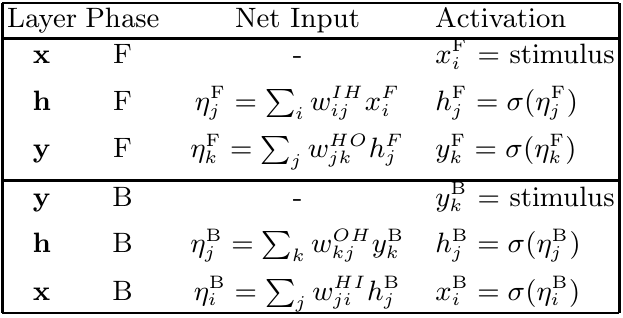
\includegraphics[scale=0.5]{img/table_bal.png} 
\citet{farkas2013bal} 
\end{center}

We avoid input-output notation of layers as used in GeneRec, because in our
case not only output can be evoked by input presentation, but also vice versa.
Hence, we label the two outer (visible) layers $x$ and $y$ and the hidden layer $h$.
Let forward activation be denoted by subscript $F$, backward activation denoted
by subscript $B$. Then during the forward pass, the $x$ units are clamped to $x^F$
and we get the activations $x^F \Rightarrow h^F \Rightarrow y^F$. During the backward pass, the $y$
units are clamped to $y^B$ and we get the activations $y^B \Rightarrow h^B \Rightarrow x^B$.

The mechanism of weights update partially matches that of GeneRec. Each
weight in BAL network (i.e. belonging to one of the four weight matrices) is
updated using the same learning mechanism, according to which the weight
difference is proportional to the product of the presynaptic (sending) unit ac-
tivation ap and the difference of postsynaptic (receiving) unit activations aq ,
corresponding to two activation phases ($F$ and $B$, in particular order). Namely,
weights in $x$-to-$y$ direction (belonging to $h$ and $y$ units) are updated as
$$
\Delta w_{pq}^F = \lambda a_p^F(a_q^B - a_q^F)
$$
where, as in the GeneRec algorithm, $a^F_p$ denotes the presynaptic activity, $a^F_q$ is the postsynaptic activity, and $a^B_q$ denotes the postsynaptic activity from the opposite phase ($y$-to-$h$). Analogically, the weights in $y$-to-$x$ direction (belonging to $h$ and $x$ units) are updated as 
$$
\Delta w_{pq}^B = \lambda a^B_p(a_q^F - a_q^B)
$$
All units have trainable thresholds (biases) that are updated in the same way
as regular weights (being fed with a constant input 1) \citet{farkas2013bal}.
 


